\documentclass[12pt]{article}
\usepackage{mwe,tikz}\usepackage[percent]{overpic}
\pagestyle{empty}

\begin{document}
\begin{figure}
  \centering   
  \begin{overpic}[scale=1.0]{../DMD-mode-79-python-test-006-crop.pdf}
     \put(5.5,40){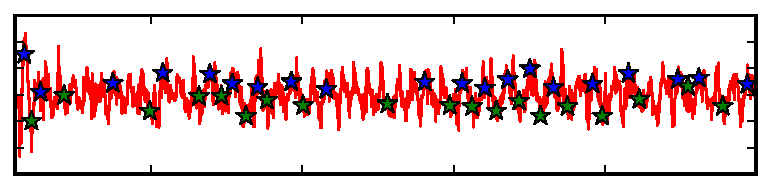
\includegraphics[scale=0.56]{../2015-10-02-11-33-DMD-mode-projection-79-timeseries.pdf}}  
  \end{overpic}
\end{figure}

%% \begin{figure} \centering
%% \begin{tikzpicture}[      
%%         every node/.style={anchor=south west,inner sep=0pt},
%%         x=1mm, y=1mm,
%%       ]   
%%      \node (fig1) at (0,0)
%%        {\includegraphics[scale=0.75]{example-image-a}};
%%      \node (fig2) at (3,3)
%%        {\includegraphics[scale=0.21]{example-image-b}};  
%% \end{tikzpicture}
%% \caption{Using Tikz Overlay}
%% \end{figure}

\end{document}
